
\chapter{Implementacija i korisničko sučelje}

	
		
		\section{Korištene tehnologije i alati}

        Timsku komunikaciju smo uspješno ostvarili kroz aplikaciju \href{https://discord.com/}{Discord}, pružajući jednostavnu i iznimno organiziranu interakciju putem "channel" i "thread" opcija. Za izradu UML dijagrama smo koristili alat \href{https://astah.net/products/astah-uml/}{Astah UML}, dok smo za upravljanje izvornim kodom primijenili \href{https://github.com/}{GitHub}.

        Kao razvojno okruženje odabrali smo \href{https://www.jetbrains.com/idea/}{IntelliJ IDEA}, integrirano razvojno okruženje (IDE) tvrtke JetBrains. Ovo okruženje pruža napredne mogućnosti kao što su dovršavanje koda analizom konteksta, navigacija koda s mogućnošću izravnog skakanja na klasu ili deklaraciju u kodu, refaktoriranje koda, rješavanje pogrešaka te ugrađene naredbe za Git, uz mnogobrojna proširenja za različite programske jezike i alate.

        Na strani klijentske aplikacije (frontend), koristili smo \href{https://reactjs.org/}{React.js}, popularnu \href{https://www.javascript.com/}{JavaScript} biblioteku za izradu korisničkih sučelja u web aplikacijama. Virtualna DOM tehnologija ovog okvira doprinosi efikasnijem ažuriranju sučelja, unaprjeđujući performanse i korisničko iskustvo.

        Za poslužiteljsku stranu aplikacije (backend) odabrali smo \href{https://spring.io/}{Spring Framework}, sveobuhvatan okvir za \href{https://www.java.com/en/}{Java} programski jezik. Poznat po konceptima inverzije kontrole i ubrizgavanja ovisnosti, Spring olakšava razvoj aplikacija pružajući modularnost, testabilnost te olakšava održavanje koda. Za upravljanje bazama podataka koristili smo \href{https://www.postgresql.org/}{PostgreSQL}, moćan objektno-relacijski sustav otvorenog koda. Njegova pouzdanost, skalabilnost i podrška za kompleksne upite čine ga optimalnim izborom za naše potrebe.
			
			\eject
		
	
		\section{Ispitivanje programskog rješenja}
			

			
			\subsection{Ispitivanje komponenti}

			 Provedbu ispitivanja implementiranih funkcionalnosti proveli smo na razini komponenti kroz detaljne unit testove. Fokusirali smo se na provjeru ispravnosti pomo- ćnih funkcija koje su ključne u različitim dijelovima koda. Ukupno smo izvršili sedam testova, a u nastavku donosimo sažete opise svakog testa zajedno s pripadajućim kodovima. Svaki opis testa popraćen je slikom koja jasno prikazuje rezultate izvođenja. Ovaj pristup omogućio nam je temeljitu analizu osnovne funkcionalnosti i identifikaciju rubnih uvjeta, pridonoseći sigurnosti i stabilnosti cijelog sustava. Nastojali smo osigurati sveobuhvatan pregled implementiranih funkcionalnosti kroz precizno definirane ispitne slučajeve.


            \subsubsection{Ispitni slučaj 1.: Test provjere svojstva dokumenta}

                        \noindent\textbf{Ulaz:}
                        \begin{packed_item}
                        	\item  Stvaranje primjerka korisnika (User) i postavljanje njegovih svojstava (ID i nadimak)
                        	\item  Stvaranje primjerka dokumenta (Document) i postavljanje njegovih svojstava (ID korisnika, korisnik, status dokumenta).
                        \end{packed_item}

                        \noindent\textbf{Očekivani rezultati:}
                        \begin{packed_item}
                        	\item  Očekujemo da će dokument imati ispravno postavljene vrijednosti svojstava, u skladu s postavljenim ulaznim podacima.
                        \end{packed_item}
                      
                        \noindent\textbf{Rezultat:}
                        \begin{packed_item}
                        	\item  Izvršavanje ovog dijela testa provjerava ispravnost postavljanja svojstava dokumenta i uspoređuje ih s očekivanim rezultatima.
                        \end{packed_item}
                       \begin{figure} [H]
                       	\centering
                       	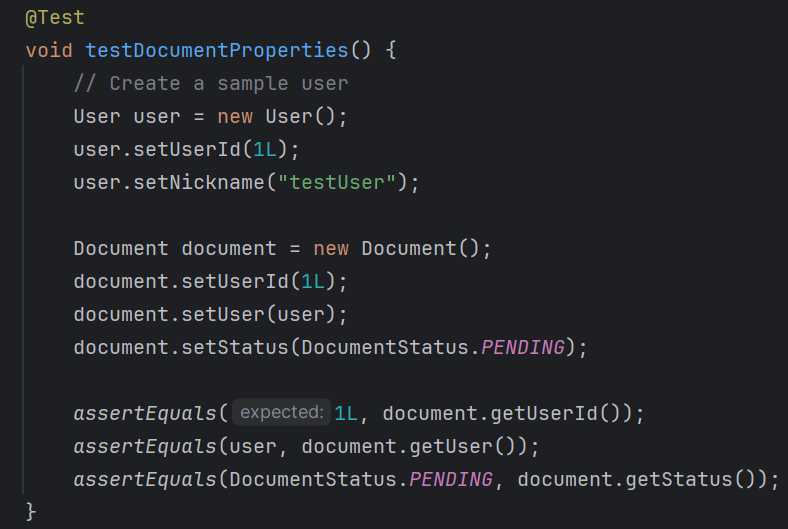
\includegraphics[width=0.7\linewidth]{slike/DokumentTest.png}
                       	\caption{Test provjere svojstva dokumenta}
                       	\label{fig:Test provjere svojstva dokumenta}
                       \end{figure}
                      



            \subsubsection{Ispitni slučaj 2.: Test provjere funkcionalnosti ImageChangeRequestStatus}

                                    \noindent\textbf{Ulaz:}
                                    \begin{packed_item}
                                    	\item Nema posebnog ulaza jer testira vrijednosti unutar samog enuma
                                    \end{packed_item}
                      
                                    \noindent\textbf{Očekivani rezultati:}
                                    \begin{packed_item}
                                    	\item Očekujemo da će vrijednosti enuma biti ispravno postavljene.
                                    	\item Očekujemo da će konverzija enuma u String biti ispravna.
                                    \end{packed_item}
                                    \noindent\textbf{Rezultat:}
                                    \begin{packed_item}
                                    	\item Izvršavanje testa provjerava da li su vrijednosti enuma ImageChangeRequestStatus ispravno postavljene
                                    	\item Izvršavanje testa provjerava da li su vrijednosti enuma ImageChangeRequestStatus ispravno postavljene
                                    \end{packed_item}
                                    
                                    
                        \begin{figure} [H]
                        	\centering
                        	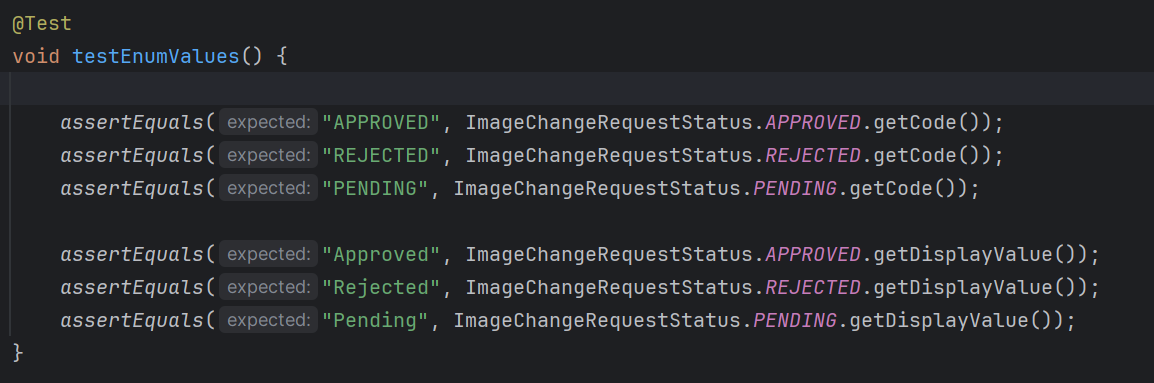
\includegraphics[width=0.7\linewidth]{slike/ImageChangeTest.png}
                        	\caption{Test provjere funkcionalnosti ImageChangeRequestStatus}
                        	\label{fig:Test provjere funkcionalnosti ImageChangeRequestStatus}
                        \end{figure}
                        
                        \begin{figure} [H]
                        	\centering
                        	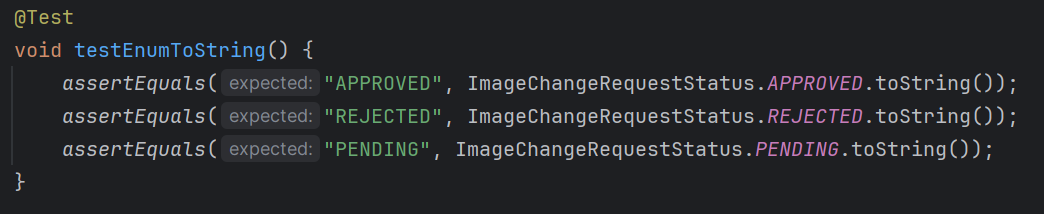
\includegraphics[width=0.7\linewidth]{slike/ImageChangeTest1.png}
                        	\caption{Test provjere funkcionalnosti ImageChangeRequestStatus}
                        	\label{fig:Test provjere funkcionalnosti ImageChangeRequestStatus}
                        \end{figure}
                                    
      

			\subsubsection{Ispitni slučaj 3.: Provjera vraćanja vremena u razredu Listing}
					\noindent\textbf{Ulaz:}
					\begin{packed_item}
						\item Stvaranje instance razreda Listing
						\item Postavljanje vremena povratka (returnByTime) na trenutno vrijeme
					\end{packed_item}
					
					\noindent\textbf{Očekivani rezultati:}
					\begin{packed_item}
						\item Očekujemo da će vrijeme povratka biti jednako trenutnom vremenu u obliku Timestamp objekta
						\item Očekujemo da će vrijednost vremena povratka biti null, budući da nije postavljena
					\end{packed_item}
					 \noindent\textbf{Rezultat:}
					\begin{packed_item}
						\item  Izvršavanje testa provjerava postavljanje i dohvaćanje vremena povratka, uspo- ređujući ga s očekivanim rezultatom
						\item  Izvršavanje testa provjerava da li je vrijednost vremena povratka null, što ukazuje na ispravno ponašanje u slučaju ne postavljanja vremena povratka
					\end{packed_item}
					
					 \begin{figure} [H]
						\centering
						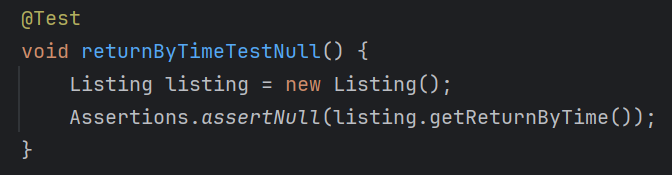
\includegraphics[width=0.7\linewidth]{slike/ListingTest.png}
						\caption{Provjera vraćanja vremena u razredu Listing}
						\label{fig:Provjera vraćanja vremena u razredu Listing}
					\end{figure}
					 \begin{figure} [H]
						\centering
						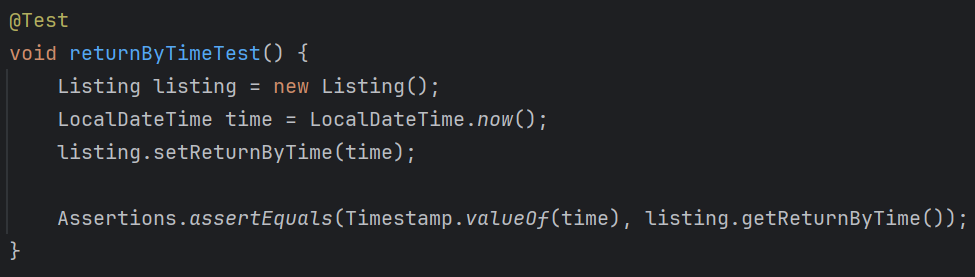
\includegraphics[width=0.7\linewidth]{slike/ListingTest1.png}
						\caption{Provjera vraćanja vremena u razredu Listing}
						\label{fig:Provjera vraćanja vremena u razredu Listing}
					\end{figure}


			\subsubsection{Ispitni slučaj 4.: Test provjere svojstava skutera}

					\noindent\textbf{Ulaz:}
					\begin{packed_item}
						\item Stvaranje primjerka korisnika (User) i postavljanje njegovih svojstava (ID i nadimak)
						\item Stvaranje primjerka skutera (Scooter) i postavljanje njegovih svojstava (ID, proizvođač, model, kapacitet baterije, maksimalna brzina, putanja do slike, maksimalni doseg, godina proizvodnje, dodatne informacije, korisnik, dostupnost)
					\end{packed_item}
					
					\noindent\textbf{Očekivani rezultati:}
					\begin{packed_item}
						\item Očekujemo da će svojstva skutera biti ispravno postavljena prema unesenim vrijednostima.
					\end{packed_item}
					\noindent\textbf{Rezultat:}
					\begin{packed_item}
						\item  Izvršavanje testa provjerava ispravnost postavljanja svojstava skutera i uspo- ređuje ih s očekivanim rezultatima.
						 postavljanja vremena povratka
					\end{packed_item}
              \begin{figure} [H]
              	\centering
              	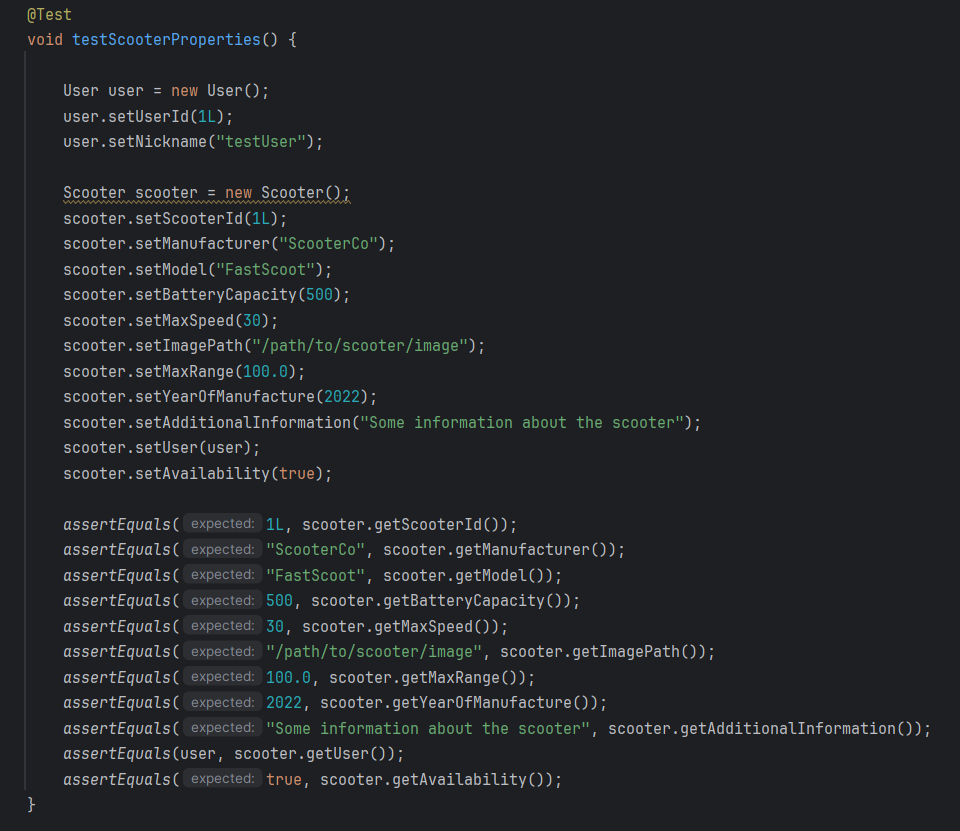
\includegraphics[width=0.7\linewidth]{slike/ScooterTest.png}
              	\caption{Test provjere svojstava skutera}
              	\label{fig:Test provjere svojstava skutera}
              \end{figure}

     
			\subsubsection{Ispitni slučaj 5.: Test provjere vremena plaćanja u razredu transakcije}
			
			
			\noindent \textbf{Ulaz:}
			\begin{packed_item}
				\item Stvaranje instance razreda Transaction
				\item Postavljanje vremena plaćanja (paymentTime) na trenutno vrijeme
			\end{packed_item}
			
			\noindent \textbf{Očekivani rezultati:}
			\begin{packed_item}
				\item Očekujemo da će vrijeme plaćanja biti jednako trenutnom vremenu u obliku Timestamp objekta
				\item Očekujemo da će vrijednost vremena plaćanja biti null, budući da nije postavljena
			\end{packed_item}
			\noindent \textbf{Rezultat:}
			\begin{packed_item}
				\item  Izvršavanje testa provjerava postavljanje i dohvaćanje vremena plaćanja, uspo- ređujući ga s očekivanim rezultatom
				\item Izvršavanje testa provjerava da li je vrijednost vremena plaćanja null, što ukazuje na ispravno ponašanje u slučaju ne postavljanja vremena plaćanja.
			\end{packed_item}
			
			\begin{figure} [H]
				\centering
				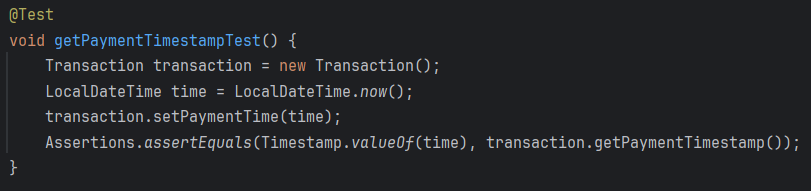
\includegraphics[width=0.7\linewidth]{slike/TransactionTest.png}
				\caption{Test provjere vremena plaćanja u razredu transakcije}
				\label{fig:Test provjere vremena plaćanja u razredu transakcije}
			\end{figure}
			\begin{figure} [H]
				\centering
				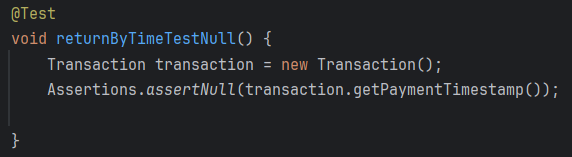
\includegraphics[width=0.7\linewidth]{slike/TransactionTest1.png}
				\caption{Test provjere vremena plaćanja u razredu transakcije}
				\label{fig:Test provjere vremena plaćanja u razredu transakcije}
			\end{figure}

                                                                      
           


            \subsubsection{Ispitni slučaj 6.: Test provjere svojstva korisnika}
            
            \noindent\textbf{Ulaz:}
            \begin{packed_item}
            	\item Stvaranje primjerka korisnika (User) i postavljanje njegovih svojstava (ID, nadimak, ime, prezime, broj kartice, e-mail, broj telefona, lozinka, uloga, status)
            \end{packed_item}
            
            \noindent\textbf{Očekivani rezultati:}
            \begin{packed_item}
            	\item Očekujemo da će svojstva korisnika biti ispravno postavljena prema unesenim vrijednostima
            \end{packed_item}
            \noindent\textbf{Rezultat:}
            \begin{packed_item}
            	\item  Izvršavanje testa provjerava ispravnost postavljanja svojstava korisnika i uspo- ređuje ih s očekivanim rezultatima
            \end{packed_item}

				\begin{figure} [H]
					\centering
					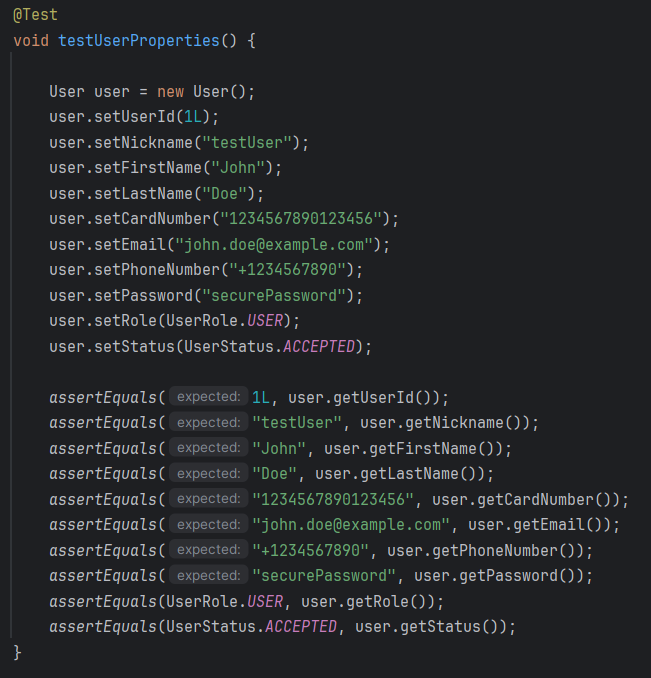
\includegraphics[width=0.7\linewidth]{slike/UserTest.png}
					\caption{Test provjere svojstva korisnika}
					\label{fig:Test provjere svojstva korisnika}
				\end{figure}

        


            \subsubsection{Ispitni slučaj 7.: Test provjere funkcionalnosti prijave korisnika}
            
             \noindent\textbf{Ulaz:}
            \begin{packed_item}
            	\item Koristi se Mock objekt UserRepository
            	\item Koristi se UserService objekt, gdje je userService injektiran u UserService pomoću @InjectMocks
            	\item Postavlja se Mock korisnik (mockUser) s podacima za prijavu
            \end{packed_item}
            
            \noindent\textbf{Očekivani rezultati:}
            \begin{packed_item}
            	\item Očekuje se da će korisničko ime i lozinka odgovarati podacima Mock korisnika
            	\item Očekuje se da će userService uspješno vratiti Mock korisnika
            	
            \end{packed_item}
            \noindent\textbf{Rezultat:}
            \begin{packed_item}
            	\item  Izvršava se prijava korisnika pomoću userService.login("test@example.com", "password")
            	\item  Provjerava se je li rezultat jednak Mock korisniku (mockUser)
            \end{packed_item}
				\begin{figure} [H]
					\centering
					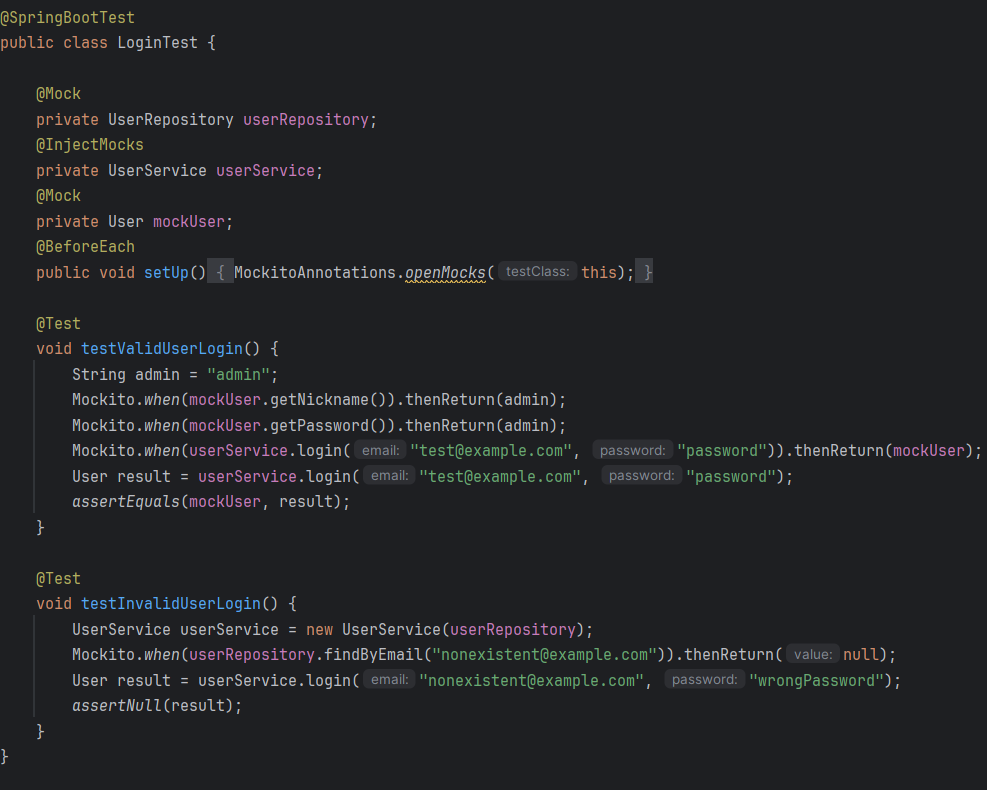
\includegraphics[width=0.7\linewidth]{slike/LoginTest.png}
					\caption{Test provjere funkcionalnosti prijave korisnika}
					\label{fig:Test provjere funkcionalnosti prijave korisnika}
				\end{figure}
                                                                                           
                       



			\subsection{Ispitivanje sustava}



			\subsubsection{Ispitni slučaj 1: Provjera ispravnosti registracije}
			
			\noindent\textbf{Cilj:}
			\begin{packed_item}
				Automatsko testiranje procesa registracije novog korisnika koji ne unese broj mobitela na web stranici pomoću Selenium WebDriver s Chrome preglednikom.
			\end{packed_item}
			
			\noindent\textbf{Koraci testiranja:}
			\begin{packed_item}
				\item Navigacija na stranicu za registraciju
				\item Ispunjavanje svih polja registracijskog obrazca osim polja za broj mobitela
				\item  Potvrda Registracije
				\item  Provjera je li se korisnik registrirao
				
			\end{packed_item}
			\noindent\textbf{Očekivani rezultati:}
			\begin{packed_item}
				\item  Korisnik se nije uspio registrirati
				\item Ispisana odgovarajuća poruka
			\end{packed_item}


						\begin{figure} [H]
							\centering
							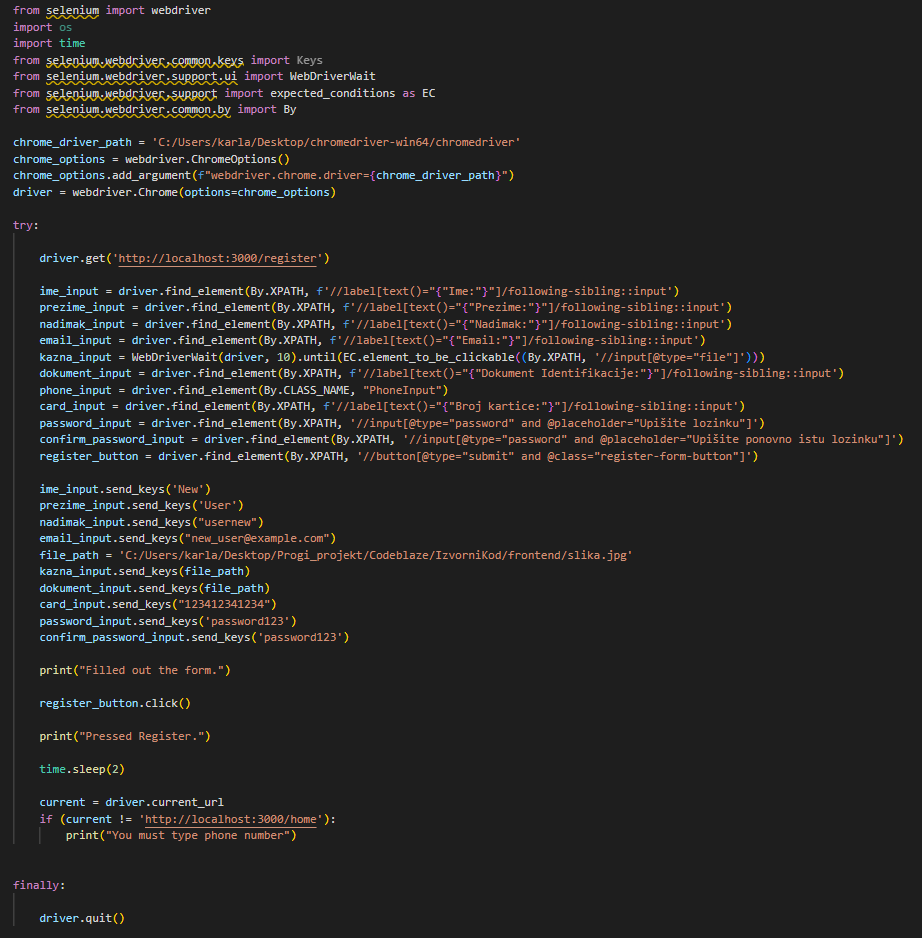
\includegraphics[width=0.7\linewidth]{slike/RegisterSelenium.png}
							\caption{Provjera ispravnosti registracije}
							\label{fig:Provjera ispravnosti registracije}
						\end{figure}
						
						\begin{figure} [H]
							\centering
							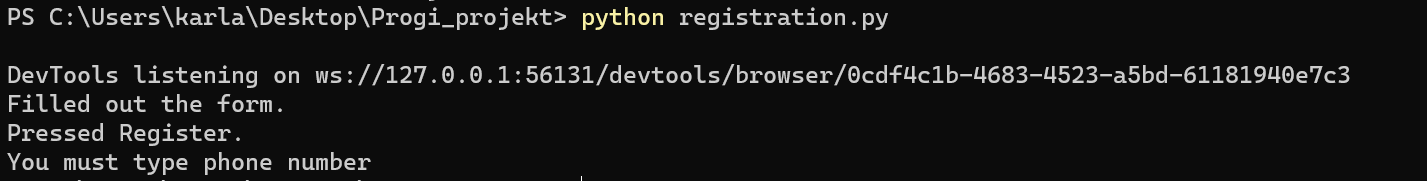
\includegraphics[width=0.7\linewidth]{slike/RegisterSeleniumOutput.png}
							\caption{Provjera ispravnosti registracije}
							\label{fig:Provjera ispravnosti registracije}
						\end{figure}

                        


            \subsubsection{Ispitni slučaj 2: Provjera ispravnosti prijave}

                        Ovaj Selenium test simulira korisničku prijavu na web stranici, unoseći korisničko ime i lozinku te provjerava očekivani rezultat, tj. naslov stranice nakon prijave.
                        
                        \noindent\textbf{Cilj:}
                        \begin{packed_item}
                        	Automatsko testiranje procesa prijavljivanja na web stranicu pomoću Selenium WebDriver s Chrome preglednikom.
                        \end{packed_item}
                        
                        \noindent\textbf{Koraci testiranja:}
                        \begin{packed_item}
                        	\item Navigacija na stranicu za prijavu
                        	\item  Unos podataka za prijavu
                        	\item Provjera stranice nakon prijave
                        	
                        \end{packed_item}
                        \noindent\textbf{Očekivani rezultati:}
                        \begin{packed_item}
                        	\item  Poruka "Assertion successful: 'Codeblaze' is in the title." ispisuje se kao potvrda uspješne prijave.
                        \end{packed_item}
                                                             

				\begin{figure} [H]
					\centering
					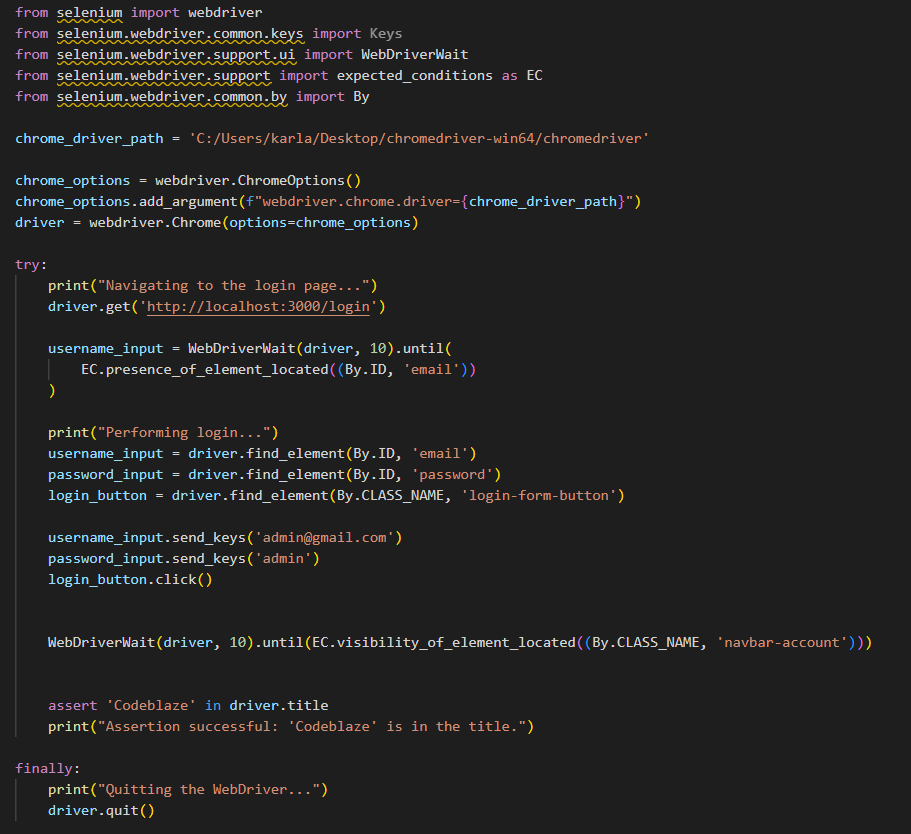
\includegraphics[width=0.7\linewidth]{slike/LoginSelenium.png}
					\caption{Provjera ispravnosti prijava}
					\label{fig:Provjera ispravnosti prijava}
				\end{figure}
				\begin{figure} [H]
					\centering
					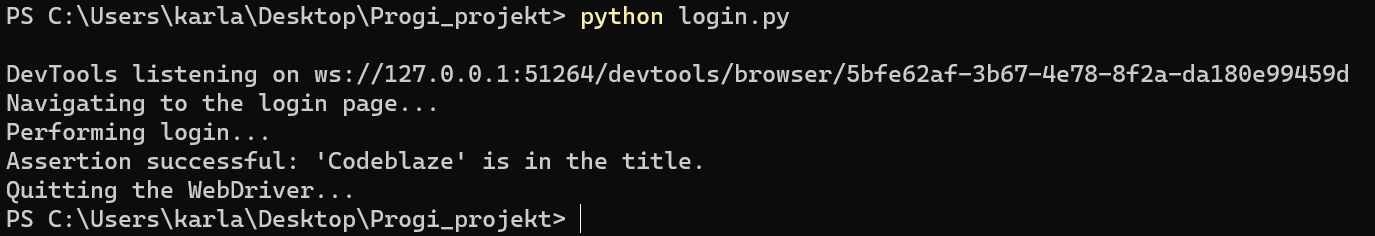
\includegraphics[width=0.7\linewidth]{slike/LoginSeleniumOutput.png}
					\caption{Provjera ispravnosti prijava}
					\label{fig:Provjera ispravnosti prijava}
				\end{figure}
                                  




			
			\eject 
		
		
		\section{Dijagram razmještaja}
			
			Dijagram rasporeda ilustrira kako su fizički i softverski resursi distribuirani unutar operativnog okvira sustava. Na serveru se smještaju dva ključna servisa: servis za web i servis za upravljanje bazom podataka. Kroz web preglednike, korisnici stječu pristup funkcionalnostima web aplikacije. Ovaj sustav funkcioniše po modelu klijent-server arhitekture gdje je komunikacijski protokol između korisničkih uređaja i servera omogućen putem HTTP veze.

		\begin{figure} [H]
			\centering
			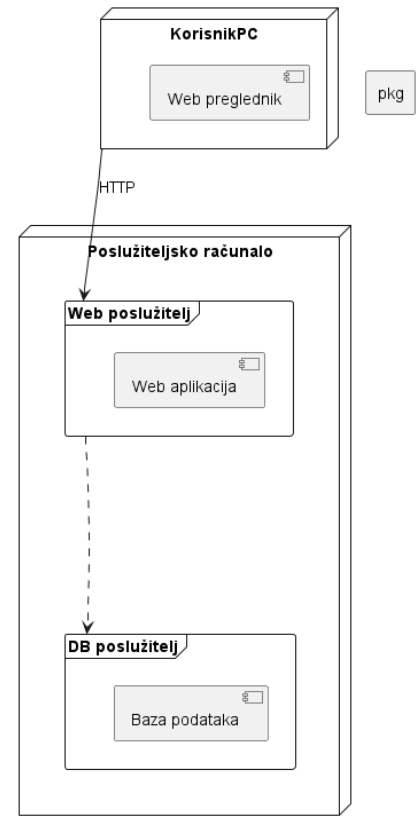
\includegraphics[width=0.7\linewidth]{dijagrami/dijagramRazmjestanja.png}
			\caption{Prikaz dijagrama razmještanja}
			\label{fig:Prikaz dijagrama razmještanja}
		\end{figure}

			\eject 
		
		\section{Upute za puštanje u pogon}


		Nakon pažljivog razvoja naše aplikacije, usmjereni smo na implementaciju u produkcijsko okruženje koristeći Render, platformu koja pruža PaaS rješenje. Ovaj proces je zahtijevao integraciju svih aplikacijskih komponenti na GitHubu, omogućujući time stvaranje Docker kontejnera, ključnih za funkcionalnost aplikacije u radnom okruženju.

		\begin{figure} [H]
			\centering
			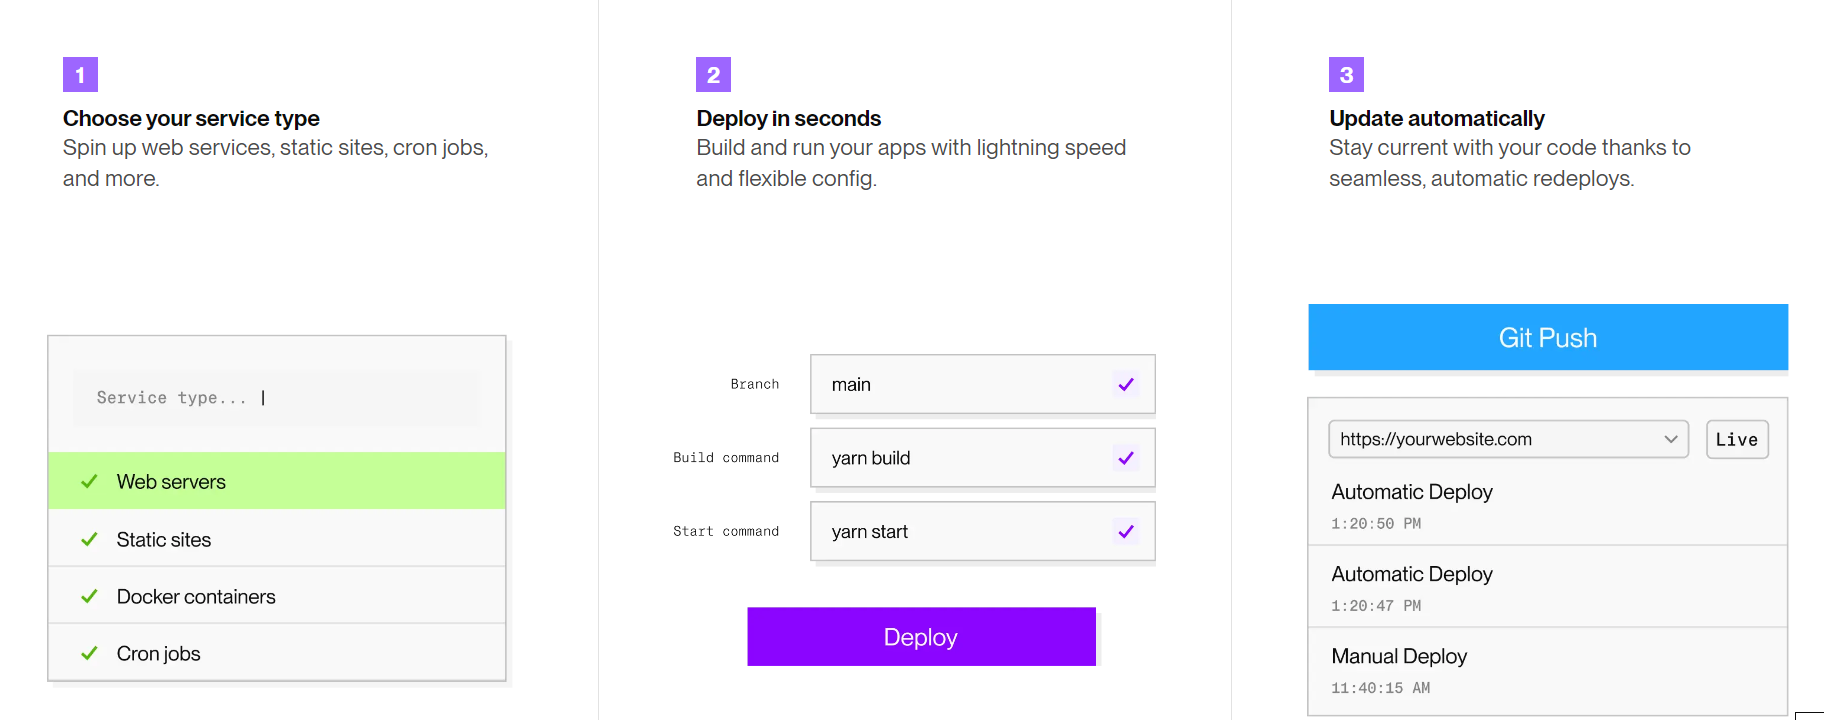
\includegraphics[width=0.7\linewidth]{slike/render.png}
			\caption{Prikaz Render platforme.}
			\label{fig:Prikaz Render platforme.}
		\end{figure}

		Pregledom izvornog koda na GitHub repozitoriju osigurali smo praćenje i upravljanje verzijama koda. Izvorni kod naše aplikacije dostupan je na https://github.com/Kvesa- Fer/Codeblaze. Prilikom pripreme za deploy, pažljivo smo postavili environment varijable u konfiguraciju našeg IDE-a kako bismo osigurali nesmetano funkcioniranje lokalnog razvojnog okruženja. Posebna pažnja posvećena je Dockerfile-u, gdje smo se pobrinuli da putanje unutar COPY naredbi budu precizno definirane.

		Konfiguracijska datoteka application.properties sadrži ključne informacije za povezivanje s bazom podataka. U razvojnom okruženju, koristili smo H2 in-memory bazu, što je vidljivo iz konfiguracije spring.datasource parametara koji ukazuju na H2 bazu. Za produkcijsko okruženje, komentirane linije sadrže konfiguraciju za povezivanje s PostgreSQL bazom podataka hostiranom na Renderu.

		Dodatno, omogućili smo pristup H2 konzoli postavljanjem spring.h2.console.enabled na true, što olakšava debugiranje i testiranje aplikacije u razvoju. Secret key, definiran u application.properties, koristi se za JWT autentifikaciju, dok logiranje različitih komponenti aplikacije postavljamo na odgovarajuće razine za detaljno praćenje tijekom razvoja i debugiranja.

		\begin{figure} [H]
			\centering
			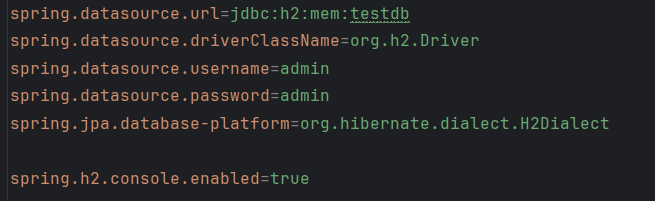
\includegraphics[width=0.7\linewidth]{slike/ap.png}
			\caption{Lokalni razvoj (koristeći H2 bazu).}
			\label{fig:Lokalni razvoj (koristeći H2 bazu).}
		\end{figure}

		Dockerfile.txt sadrži naredbe za kreiranje Docker slike aplikacije. Korištenjem dvostupanjskog procesa izgradnje, prvo se stvara build container koji izvršava Maven build, a zatim se finalna izvršna JAR datoteka kopira u runtime container.

		\begin{figure} [H]
			\centering
			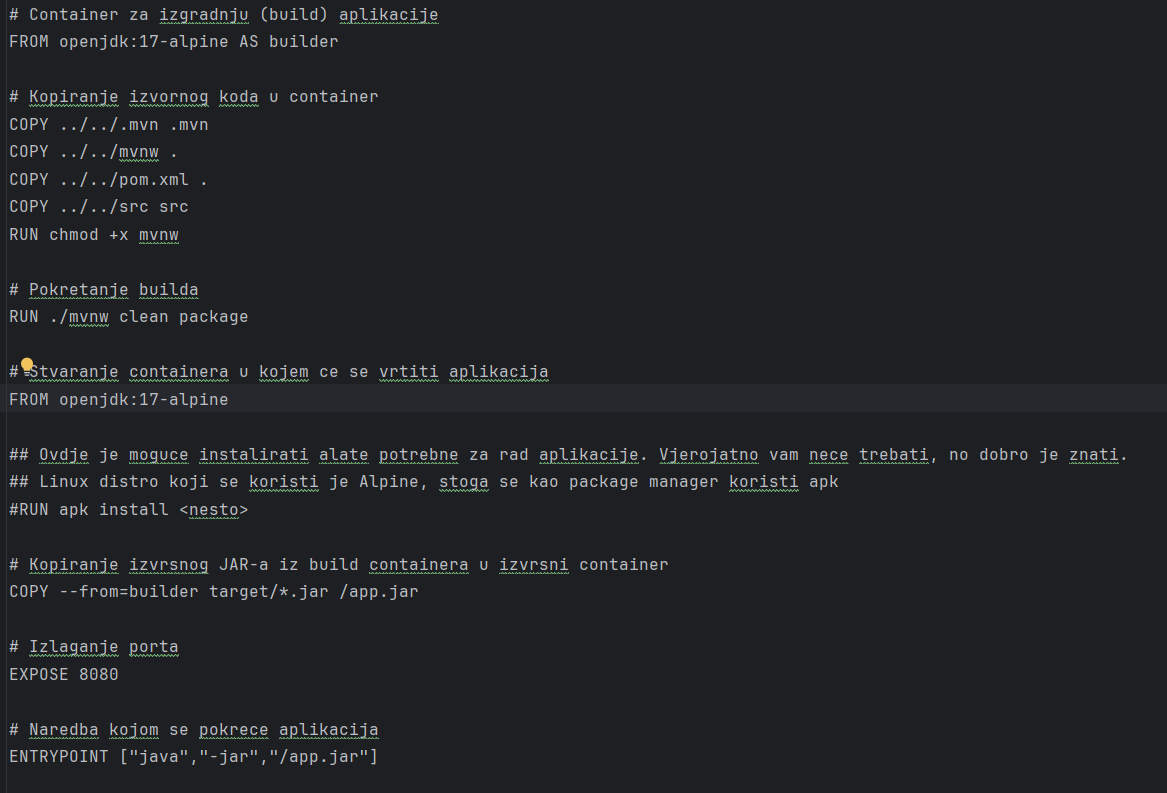
\includegraphics[width=0.7\linewidth]{slike/docker.png}
			\caption{Izgradnja i konfiguracija Docker kontejnera}
			\label{fig:Izgradnja i konfiguracija Docker kontejnera}
		\end{figure}

		setupproxy.js definira proxy middleware koji preusmjerava zahtjeve na /api endpointu na backend server, što omogućuje jednostavniju integraciju frontend i backend dijelova aplikacije tijekom razvoja.

		\begin{figure} [H]
			\centering
			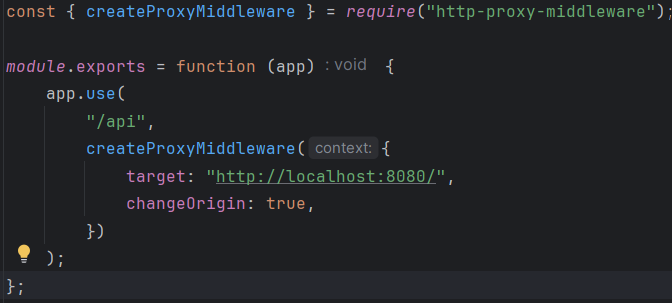
\includegraphics[width=0.7\linewidth]{slike/setupproxy.png}
			\caption{Konfiguracija proxy middlewarea za preusmjeravanje API zahtjeva}
			\label{fig:Konfiguracija proxy middlewarea za preusmjeravanje API zahtjeva}
		\end{figure}

		package.json definira metapodatke projekta, dependency-e potrebne za frontend dio aplikacije, kao i skripte koje se koriste za pokretanje i izgradnju projekta. Vidimo i konfiguraciju Node verzije koja se koristi, što osigurava kompatibilnost između različitih razvojnih okruženja.

		\begin{figure} [H]
			\centering
			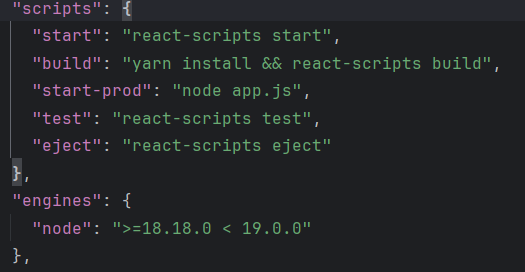
\includegraphics[width=0.7\linewidth]{slike/package.png}
			\caption{Definicija skripti za pokretanje i izgradnju projekta}
			\label{fig:Definicija skripti za pokretanje i izgradnju projekta}
		\end{figure}

		app.js postavlja express server koji služi statičke datoteke iz build direktorija i postavlja proxy za API zahtjeve. Konfiguracija se čita iz environment varijabli, što omogućuje fleksibilnost i jednostavnost konfiguracije u različitim okruženjima.

		\begin{figure} [H]
			\centering
			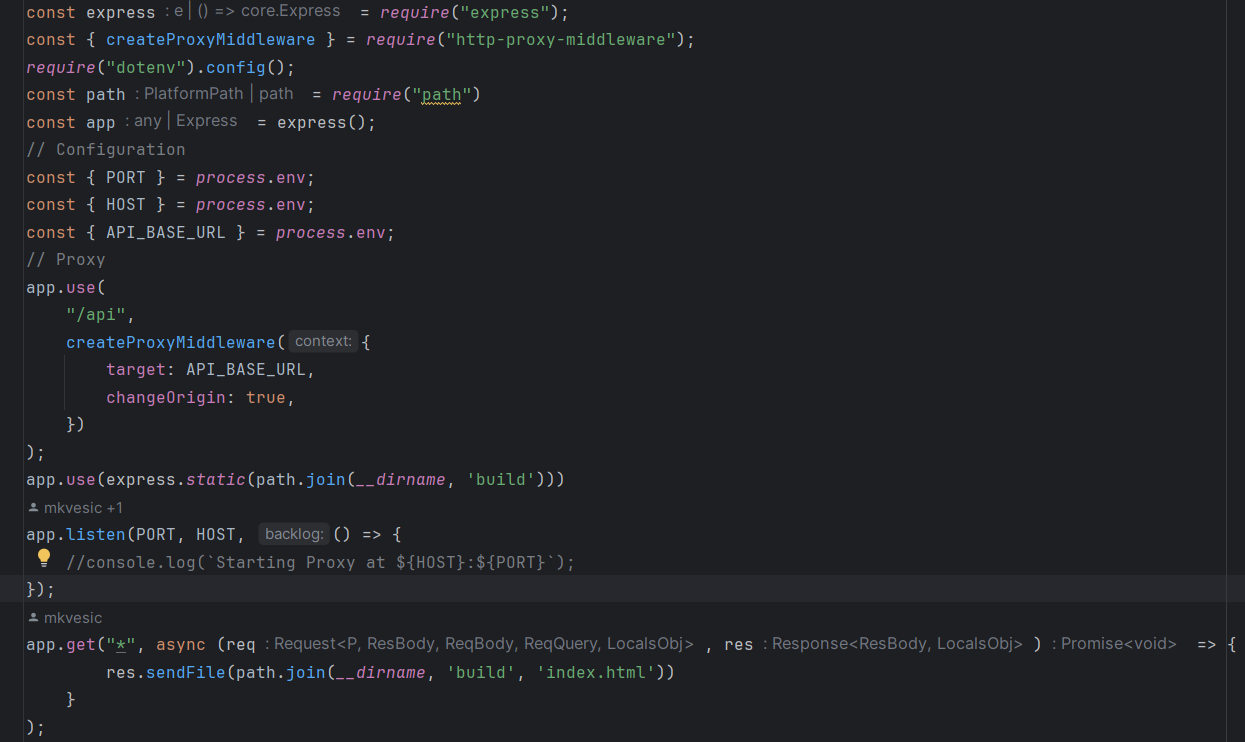
\includegraphics[width=0.7\linewidth]{slike/app.png}
			\caption{Postavljanje Express servera s proxyjem i statickim serviranjem}
			\label{fig:Postavljanje Express servera s proxyjem i statickim serviranjem}
		\end{figure}

		Kroz ovaj proces, stvorili smo stabilnu, sigurnu i skalabilnu aplikaciju spremnu za produkcijsko okruženje. Deploy aplikacije na Render platformi bio je ključan korak u dostizanju naših operativnih ciljeva, omogućujući nam da našu aplikaciju učinimo dostupnom široj publici.

		Konačna aplikacija dostupna je na poveznici: https://codeblazefe.onrender.com/home.


		\eject